% Options for packages loaded elsewhere
\PassOptionsToPackage{unicode}{hyperref}
\PassOptionsToPackage{hyphens}{url}
%
\documentclass[
  20pt,
]{book}
\usepackage{amsmath,amssymb}
\usepackage{iftex}
\ifPDFTeX
  \usepackage[T1]{fontenc}
  \usepackage[utf8]{inputenc}
  \usepackage{textcomp} % provide euro and other symbols
\else % if luatex or xetex
  \usepackage{unicode-math} % this also loads fontspec
  \defaultfontfeatures{Scale=MatchLowercase}
  \defaultfontfeatures[\rmfamily]{Ligatures=TeX,Scale=1}
\fi
\usepackage{lmodern}
\ifPDFTeX\else
  % xetex/luatex font selection
\fi
% Use upquote if available, for straight quotes in verbatim environments
\IfFileExists{upquote.sty}{\usepackage{upquote}}{}
\IfFileExists{microtype.sty}{% use microtype if available
  \usepackage[]{microtype}
  \UseMicrotypeSet[protrusion]{basicmath} % disable protrusion for tt fonts
}{}
\makeatletter
\@ifundefined{KOMAClassName}{% if non-KOMA class
  \IfFileExists{parskip.sty}{%
    \usepackage{parskip}
  }{% else
    \setlength{\parindent}{0pt}
    \setlength{\parskip}{6pt plus 2pt minus 1pt}}
}{% if KOMA class
  \KOMAoptions{parskip=half}}
\makeatother
\usepackage{xcolor}
\usepackage{color}
\usepackage{fancyvrb}
\newcommand{\VerbBar}{|}
\newcommand{\VERB}{\Verb[commandchars=\\\{\}]}
\DefineVerbatimEnvironment{Highlighting}{Verbatim}{commandchars=\\\{\}}
% Add ',fontsize=\small' for more characters per line
\usepackage{framed}
\definecolor{shadecolor}{RGB}{248,248,248}
\newenvironment{Shaded}{\begin{snugshade}}{\end{snugshade}}
\newcommand{\AlertTok}[1]{\textcolor[rgb]{0.94,0.16,0.16}{#1}}
\newcommand{\AnnotationTok}[1]{\textcolor[rgb]{0.56,0.35,0.01}{\textbf{\textit{#1}}}}
\newcommand{\AttributeTok}[1]{\textcolor[rgb]{0.13,0.29,0.53}{#1}}
\newcommand{\BaseNTok}[1]{\textcolor[rgb]{0.00,0.00,0.81}{#1}}
\newcommand{\BuiltInTok}[1]{#1}
\newcommand{\CharTok}[1]{\textcolor[rgb]{0.31,0.60,0.02}{#1}}
\newcommand{\CommentTok}[1]{\textcolor[rgb]{0.56,0.35,0.01}{\textit{#1}}}
\newcommand{\CommentVarTok}[1]{\textcolor[rgb]{0.56,0.35,0.01}{\textbf{\textit{#1}}}}
\newcommand{\ConstantTok}[1]{\textcolor[rgb]{0.56,0.35,0.01}{#1}}
\newcommand{\ControlFlowTok}[1]{\textcolor[rgb]{0.13,0.29,0.53}{\textbf{#1}}}
\newcommand{\DataTypeTok}[1]{\textcolor[rgb]{0.13,0.29,0.53}{#1}}
\newcommand{\DecValTok}[1]{\textcolor[rgb]{0.00,0.00,0.81}{#1}}
\newcommand{\DocumentationTok}[1]{\textcolor[rgb]{0.56,0.35,0.01}{\textbf{\textit{#1}}}}
\newcommand{\ErrorTok}[1]{\textcolor[rgb]{0.64,0.00,0.00}{\textbf{#1}}}
\newcommand{\ExtensionTok}[1]{#1}
\newcommand{\FloatTok}[1]{\textcolor[rgb]{0.00,0.00,0.81}{#1}}
\newcommand{\FunctionTok}[1]{\textcolor[rgb]{0.13,0.29,0.53}{\textbf{#1}}}
\newcommand{\ImportTok}[1]{#1}
\newcommand{\InformationTok}[1]{\textcolor[rgb]{0.56,0.35,0.01}{\textbf{\textit{#1}}}}
\newcommand{\KeywordTok}[1]{\textcolor[rgb]{0.13,0.29,0.53}{\textbf{#1}}}
\newcommand{\NormalTok}[1]{#1}
\newcommand{\OperatorTok}[1]{\textcolor[rgb]{0.81,0.36,0.00}{\textbf{#1}}}
\newcommand{\OtherTok}[1]{\textcolor[rgb]{0.56,0.35,0.01}{#1}}
\newcommand{\PreprocessorTok}[1]{\textcolor[rgb]{0.56,0.35,0.01}{\textit{#1}}}
\newcommand{\RegionMarkerTok}[1]{#1}
\newcommand{\SpecialCharTok}[1]{\textcolor[rgb]{0.81,0.36,0.00}{\textbf{#1}}}
\newcommand{\SpecialStringTok}[1]{\textcolor[rgb]{0.31,0.60,0.02}{#1}}
\newcommand{\StringTok}[1]{\textcolor[rgb]{0.31,0.60,0.02}{#1}}
\newcommand{\VariableTok}[1]{\textcolor[rgb]{0.00,0.00,0.00}{#1}}
\newcommand{\VerbatimStringTok}[1]{\textcolor[rgb]{0.31,0.60,0.02}{#1}}
\newcommand{\WarningTok}[1]{\textcolor[rgb]{0.56,0.35,0.01}{\textbf{\textit{#1}}}}
\usepackage{longtable,booktabs,array}
\usepackage{calc} % for calculating minipage widths
% Correct order of tables after \paragraph or \subparagraph
\usepackage{etoolbox}
\makeatletter
\patchcmd\longtable{\par}{\if@noskipsec\mbox{}\fi\par}{}{}
\makeatother
% Allow footnotes in longtable head/foot
\IfFileExists{footnotehyper.sty}{\usepackage{footnotehyper}}{\usepackage{footnote}}
\makesavenoteenv{longtable}
\usepackage{graphicx}
\makeatletter
\def\maxwidth{\ifdim\Gin@nat@width>\linewidth\linewidth\else\Gin@nat@width\fi}
\def\maxheight{\ifdim\Gin@nat@height>\textheight\textheight\else\Gin@nat@height\fi}
\makeatother
% Scale images if necessary, so that they will not overflow the page
% margins by default, and it is still possible to overwrite the defaults
% using explicit options in \includegraphics[width, height, ...]{}
\setkeys{Gin}{width=\maxwidth,height=\maxheight,keepaspectratio}
% Set default figure placement to htbp
\makeatletter
\def\fps@figure{htbp}
\makeatother
\setlength{\emergencystretch}{3em} % prevent overfull lines
\providecommand{\tightlist}{%
  \setlength{\itemsep}{0pt}\setlength{\parskip}{0pt}}
\setcounter{secnumdepth}{5}
\ifLuaTeX
\usepackage[bidi=basic]{babel}
\else
\usepackage[bidi=default]{babel}
\fi
\babelprovide[main,import]{spanish}
% get rid of language-specific shorthands (see #6817):
\let\LanguageShortHands\languageshorthands
\def\languageshorthands#1{}
\usepackage{booktabs}
 % \usepackage{polyglossia}
 % \setmainlanguage{spanish}
 % \usepackage{enumerate}
 % \usepackage{xcolor}

\ifxetex
  \usepackage{polyglossia}
  \setmainlanguage{spanish}
  % Tabla en lugar de cuadro
  \gappto\captionsspanish{\renewcommand{\tablename}{Tabla}
          \renewcommand{\listtablename}{Índice de tablas}}
\else
  \usepackage[spanish,es-tabla]{babel}
\fi


\ifLuaTeX
  \usepackage{selnolig}  % disable illegal ligatures
\fi
\usepackage[]{natbib}
\bibliographystyle{plainnat}
\usepackage{bookmark}
\IfFileExists{xurl.sty}{\usepackage{xurl}}{} % add URL line breaks if available
\urlstyle{same}
\hypersetup{
  pdftitle={Datos Extremales (2025)},
  pdfauthor={MEDIA},
  pdflang={es},
  hidelinks,
  pdfcreator={LaTeX via pandoc}}

\title{Datos Extremales (2025)}
\author{MEDIA}
\date{2025-03-13}

\usepackage{amsthm}
\newtheorem{theorem}{Teorema}[chapter]
\newtheorem{lemma}{Lema}[chapter]
\newtheorem{corollary}{Corolario}[chapter]
\newtheorem{proposition}{Proposición}[chapter]
\newtheorem{conjecture}{Conjecture}[chapter]
\theoremstyle{definition}
\newtheorem{definition}{Definición}[chapter]
\theoremstyle{definition}
\newtheorem{example}{Ejemplo}[chapter]
\theoremstyle{definition}
\newtheorem{exercise}{Ejercicio}[chapter]
\theoremstyle{definition}
\newtheorem{hypothesis}{Hypothesis}[chapter]
\theoremstyle{remark}
\newtheorem*{remark}{Nota: }
\newtheorem*{solution}{Solución}
\begin{document}
\maketitle

{
\setcounter{tocdepth}{1}
\tableofcontents
}
\chapter{La teoría asintótica clásica, las distribuciones extremales y sus dominios de atracción}\label{la-teoruxeda-asintuxf3tica-cluxe1sica-las-distribuciones-extremales-y-sus-dominios-de-atracciuxf3n}

\section{Datos extremos}\label{datos-extremos}

Se dice que tenemos \emph{datos extremos} cuando cada
dato corresponde al máximo o mínimo de varios
registros. Ejemplos de este tipo de datos son:

\begin{itemize}
\tightlist
\item
  La máxima altura semanal de la ola en una
  plataforma marina o portuaria \((m)\).
\item
  La máxima velocidad de viento en determinada
  dirección a lo largo de un mes \((km/h)\).
\item
  La temperatura ambiental mínima a lo largo de
  un día \((\dot{C})\).
\item
  La temperatura ambiental mínima a lo largo de
  un día (\(\dot{C}\))
\item
  La máxima velocidad de tráfico en un enlace de
  una red de datos de datos en una hora (\(Mb/s\)).
\item
  El mayor registro en un conteo de Coliformes
  fecales sobre agua costeras al cabo de quince días.
\end{itemize}

Son un caso particular de evento raro o gran
desviación respecto a la media.
En resumen, en una gran variedad de dominios
disciplinares suele ser de gran interés el trabajo
con datos extremos, los que admiten diversos
enfoques. Entre ellos, los propios al párrafo
anterior (eventos raros, grandes desviaciones), que
se verán en el curso.
Sin embargo, el comienzo del curso se centra en la
teoría más clásica de estadística de datos extremos,
basada en el trabajo de Fréchet, Gumbel, Weibull,
Fisher, Tippett, Gnedenko, entre otros.

\textbf{Observación 1:} Se recuerda que si \(X\) e \(Y\) son variables aleatorias independientes, cuyas
distribuciones son, respectivamente, \(F\) y \(G\),
entonces la variable

\begin{equation}
\max \left( X,Y \right)
\label{eq:1}
\end{equation}

tiene por distribución la función \(H\) definida por

\begin{equation}
H(t)= F(t)\; G(t)
\label{eq:2}
\end{equation}

\textbf{Observación 2:} En esta parte inicial del curso
asumiremos que nuestros datos son \(iid\)
(independientes e idénticamente distribuidos, son
dos suposiciones juntas). Esta doble suposición
suele NO ser realista en aplicaciones concretas
(ninguna de sus dos componentes, incluso) pero
para comenzar a entender la teoría clásica, la
utilizaremos por un tiempo.

\textbf{Observación 3:} Resulta claramente de la
Observación 1, que si tenemos datos \(X_1,...,X_n\) \(iid\) con distribución \(F\), entonces

\begin{equation}
X_n^{\ast}= \max \left( X_1,...,X_n \right)
\end{equation}

tiene distribución \(F_n^\ast\) dada por

\begin{equation}
F_n^\ast (t) = F(t)^n
\end{equation}

Si conocemos la distribución \(F\) conoceríamos la
distribución \(F_n^\ast\), pero en algunos casos la lectura
que queda registrada es la del dato máximo y no la
de cada observación que dio lugar al mismo, por lo
que a veces ni siquiera es viable estimar \(F\).
Pero aún en los casos en que \(F\) es conocida o
estimable, si \(n\) es grande, la fórmula de \(F_n^\ast\) puede resultar prácticamente inmanejable. En una línea de trabajo similar a la que aporta el \emph{Teorema
Central del Límite} en la estadística de valores
medios, un teorema nos va a permitir aproximar
\(F_n^\ast\) por distribuciones más sencillas. Este es el
\emph{Teorema de Fischer-Tippet-Gnedenko} (FTG) que presentaremos en breve.

\textbf{Observación 4:} Si \(X_1,...,X_n\;\) es \(iid\;\) y definimos
\(\;Y_i = -X_i\;\) para todo valor de \(i\), entonces \(Y_1,...,Y_n\;\) es \(iid\;\) y además

\begin{equation}
min(X_1,...,X_n) = - max(Y_1,...,Y_n)
\end{equation}

la teoría asintótica de los mínimos de datos \(iid\)
se reduce a la de los máximos, razón por la que
nos concentramos aquí en estudiar el
comportamiento asintótico de los \textbf{máximos}
exclusivamente.

\section{Las distribuciones extremales}\label{las-distribuciones-extremales}

Las distribuciones extremales son tres: la
\emph{distribución de Gumbel}, la \emph{distribución de Weibull} y
la \emph{distribución de Fréchet}. En su versión \emph{standard} o \emph{típica} se definen del modo
siguiente.

Se dice que una variable tiene distribución de:

-\textbf{Gumbel} si su distribución es

\[\Lambda(x) = e^{\{-e^{-x}\}}\hspace{0.3cm}\text{ para todo }\: x \;\text{real}.\]

-\textbf{Weibull} de orden \(\alpha>0\) si su distribución es

\[\Psi_{\alpha}(x)=\begin{cases}
e^{\left\{-(-x)^{\alpha}  \right\}} & si\;x<0\\
1 & \text{en otro caso}
\end{cases}\]

-\textbf{Fréchet} de orden \(\alpha>0\) si su distribución es

\[
\Phi_{\alpha}(x)=\begin{cases}
e^{\left\{ -x^{-\alpha}\right\}} & si\;x>0\\
0 & \text{en otro caso}
\end{cases}
\]
\textbf{Nota:} Como los máximos en general son valores grandes,
importa particularmente observar el comportamiento de estas distribuciones para \(x\) tendiendo a infinito. El límite es \(1\) como en toda distribución. Pero \emph{VA MAS RAPIDO} a 1 la Weibull, luego la Gumbel y luego la Fréchet. Esto es indicio que la
Fréchet modela datos \emph{más extremos}, máximos de datos de
colas más pesadas que la Gumbel y ésta que la Weibull. Más
adelante veremos esto más precisamente. En la Fréchet, la
velocidad de convergencia a 1 crece al aumentar el orden. En cambio en la Weibull el orden afecta la velocidad con que va a 0 cuando \(x\) tiende a menos infinito, que crece cuanto mayor el orden. Esto quedará más claro con el Teorema 1 del curso. La visualización de las densidades de cada tipo quizás ayude a comprender mejor los pesos relativos de las colas.

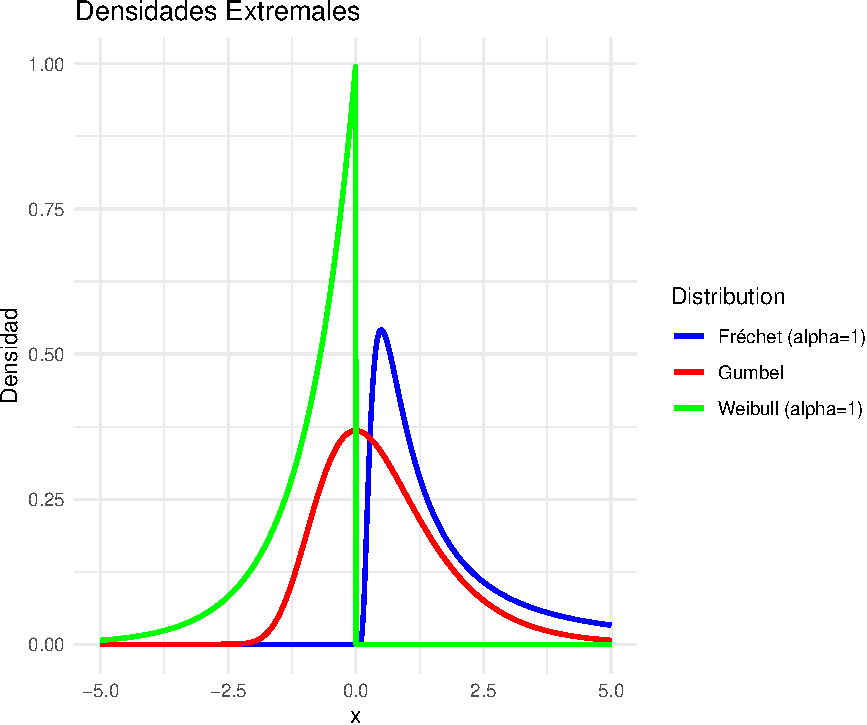
\includegraphics{Extremales_files/figure-latex/plot-extreme-distributions-1.pdf}

A estas versiones standard se las puede extender
agregando un parámetro de recentramiento \((\mu)\) y
un parámetro de escala \((\beta)\).

Se dice que \(X\) tiene distribución:

\begin{itemize}
\item
  \textbf{Gumbel} : \(\Lambda^{(\mu, \beta)}\) si \(\;X=\mu + \beta Y\;\), donde \(Y\) tiene distribución \(\Lambda\).
\item
  \textbf{Weibull}: \(\;\Psi^{(\mu, \beta)}\;\) si \(\;X=\mu + \beta Y\;\), donde \(Y\) tiene distribución \(\Psi_{\alpha}\).
\item
  \textbf{Fréchet}: \(\;\Phi^{(\mu, \beta)}\;\) si \(X=\mu + \beta Y\), donde \(Y\) tiene distribución \(\Phi_{\alpha}\).
\end{itemize}

En general, es en este sentido que diremos que una
variable es Gumbel, Weibull o Fréchet (incluyendo
recentramiento y reescalamiento), pero en cálculos
donde los parámetros \(\mu\) y \(\beta\) no sean relevantes, por
simplicidad, usaremos las versiones standard.

El siguiente teorema vincula las distribuciones
extremales en sus formatos standard y resulta de
gran utilidad práctica sobre todo al hacer tests de
ajustes, etc.

\begin{theorem}[Relaciones entre las versiones standard de las distribuciones extremales]
\protect\hypertarget{thm:foo1}{}\label{thm:foo1}\(X\) tiene distribución \(\Phi_{\alpha}\) \(\Leftrightarrow\) \((-1/X)\) tiene distribución \(\Psi_{\alpha}\) \(\Leftrightarrow\) \(\log(X^{\alpha})\) tiene distribución \(\Lambda\).
\end{theorem}

Nota: en otros contextos de la Estadística (en particular en
alguna rutinas del R), se le llama Weibull a una variable que
corresponde a -X, con X Weibull como definimos nosotros.

\textbf{Observación 5:} Recordamos que la función
Gamma (\(\Gamma\) ), que extiende a la función factorial
(\(\Gamma(n)=n-1!\quad \forall n\) natural) definida por

\begin{equation}
\Gamma(x)=\int_{0}^{\infty} t^{u-1}e^{-t}dt
\end{equation}

es una función disponible tanto en el software R
como en planillas de cálculo, etc.

\begin{theorem}[Algunos datos de las distribuciones extremales]
\protect\hypertarget{thm:foo2}{}\label{thm:foo2}

Tres partes:

\textbf{Parte 1}

Si \(X\) tiene distribución \(\Lambda^{(\mu,\beta)}\) entonces tiene:

\begin{enumerate}
\def\labelenumi{\alph{enumi})}
\item
  \textbf{Esperanza}: \(E(X) = \mu + \beta\gamma\), donde \(\gamma\) es la constante de Euler-Mascheroni, cuyo valor aproximado es \(0.5772156649\).
\item
  \textbf{Moda}: \(\text{moda}(X)=\mu\)
\item
  \textbf{Mediana}: \(\text{med}(X)=\mu - \beta \log(\log 2) \approx \mu - 0.36651 \beta\)
\item
  \textbf{Desviación estándar}: \(\sigma(X)=\frac{\beta \pi}{\sqrt{6}}   \approx 1.2825 \beta\)
\item
  Si \(X^+ = \max(X,0)\), entonces \(E(X+k)\) es finito para todo valor de \(k\) natural
\item
  Para simular computacionalmente \(X\), se puede tomar \(U\) uniforme en \((0,1)\) y hacer \(X = \mu - \beta \log(-\log U)\).
\end{enumerate}

\textbf{Parte 2}

Si \(X\) tiene distribución \(\Psi^{(\mu, \beta)}\) entonces tiene:

\begin{enumerate}
\def\labelenumi{\alph{enumi})}
\item
  \(E(X)=\mu -\beta \Gamma (1+1/\alpha)\)
\item
  \begin{equation*}\text{moda}(X) =\begin{cases} 
    \mu  & \text{si }\; \alpha \leq 1 \\
   \mu-\beta\left\{ \frac{\left( \alpha-1 \right)}{\alpha} \right\}^{1/\alpha} & \text{si }\; \alpha >1
  \end{cases}\end{equation*}
\item
  \(\text{med}(X)=\mu - \beta (\log 2)^{\frac{1}{\alpha}}\)
\item
  \(\sigma(X)=\beta\left\{\Gamma\left( 1+\frac{2}{\alpha} \right)-\Gamma\left( 1+\frac{1}{\alpha} \right)^2  \right\}^{1/2}\).
\end{enumerate}

\textbf{Parte 3}

Si \(X\) tiene distribución \(\Phi_{\alpha}^{(\mu, \beta)}\) entonces tiene:

\begin{enumerate}
\def\labelenumi{\alph{enumi})}
\item
  \begin{equation*}
  E(x) =
  \begin{cases} 
   \mu + \beta\;\Gamma\left( 1-\frac{1}{\alpha} \right) & \text{si } \alpha>1 \\
   \infty & \text{en otro caso}
  \end{cases}
  \end{equation*}
\item
  \(\text{moda}(X)=\mu+ \beta\;\left\{ \frac{\alpha}{\left( 1+ \alpha\right)}\right\}^{1/\alpha}\)
\item
  \(\text{med}(X)=\mu + \beta \;\left( \log 2 \right)^{\left( -1/\alpha \right)}\)
\item
  \begin{equation*}
  \sigma(x) =
  \begin{cases} 
   \mu + \left| \Gamma \left( 1 - \frac{2}{\alpha} \right) - \Gamma \left(  1 - \frac{1}{\alpha}\right)\right|  & \text{si } \; \alpha>2 \\
   \infty & \text{si } \; 1<\alpha \leq 2
  \end{cases}
  \end{equation*}
\end{enumerate}

\end{theorem}

\textbf{Observación 6:} El item e) de la Parte 1 es
trivialmente cierto para Weibull y tomando en
cuenta el item a) de la Parte 3, es claramente falso
para Fréchet.

\textbf{Observación 7:} El item f) de la Parte 1 en
conjunto con el teorema \ref{thm:foo1} brinda fórmulas
sencillas para simular computacionalmente
distribuciones Weibull o Fréchet.

\textbf{Observación 8:} Se generaron mil números aleatorios y aplicando el
item f) de la Parte 1: se simularon mil variables
Gumbel standard \(iid\), calculándose su promedio, su
desviación standard empírica y su mediana
empírica.

\begin{Shaded}
\begin{Highlighting}[]
\CommentTok{\# Fijar semilla para reproducibilidad}
\FunctionTok{set.seed}\NormalTok{(}\DecValTok{123}\NormalTok{)}

\CommentTok{\# Definir parámetros}
\NormalTok{mu }\OtherTok{\textless{}{-}} \DecValTok{0}       \CommentTok{\# Centro}
\NormalTok{beta }\OtherTok{\textless{}{-}} \DecValTok{1}     \CommentTok{\# Escala}
\NormalTok{gamma }\OtherTok{\textless{}{-}} \FloatTok{0.5772156649}  \CommentTok{\# Constante de Euler{-}Mascheroni}

\CommentTok{\# Número de simulaciones}
\NormalTok{n }\OtherTok{\textless{}{-}} \DecValTok{1000}

\CommentTok{\# Generar 1000 valores de una variable uniforme en (0,1)}
\NormalTok{U }\OtherTok{\textless{}{-}} \FunctionTok{runif}\NormalTok{(n)}

\CommentTok{\# Simular la variable Gumbel con parámetros (mu, beta)}
\NormalTok{X\_gumbel }\OtherTok{\textless{}{-}}\NormalTok{ mu }\SpecialCharTok{{-}}\NormalTok{ beta }\SpecialCharTok{*} \FunctionTok{log}\NormalTok{(}\SpecialCharTok{{-}}\FunctionTok{log}\NormalTok{(U))}

\CommentTok{\# Calcular estadísticas}
\NormalTok{esperanza }\OtherTok{\textless{}{-}}\NormalTok{ mu }\SpecialCharTok{+}\NormalTok{ beta }\SpecialCharTok{*}\NormalTok{ gamma}
\NormalTok{moda }\OtherTok{\textless{}{-}}\NormalTok{ mu}
\NormalTok{mediana\_teorica }\OtherTok{\textless{}{-}}\NormalTok{ mu }\SpecialCharTok{{-}}\NormalTok{ beta }\SpecialCharTok{*} \FunctionTok{log}\NormalTok{(}\FunctionTok{log}\NormalTok{(}\DecValTok{2}\NormalTok{))}
\NormalTok{desviacion\_std\_teorica }\OtherTok{\textless{}{-}}\NormalTok{ beta }\SpecialCharTok{*}\NormalTok{ pi }\SpecialCharTok{/} \FunctionTok{sqrt}\NormalTok{(}\DecValTok{6}\NormalTok{)}

\CommentTok{\# Calcular estadísticas empíricas}
\NormalTok{promedio\_empirico }\OtherTok{\textless{}{-}} \FunctionTok{mean}\NormalTok{(X\_gumbel)}
\NormalTok{desviacion\_std\_empirica }\OtherTok{\textless{}{-}} \FunctionTok{sd}\NormalTok{(X\_gumbel)}
\NormalTok{mediana\_empirica }\OtherTok{\textless{}{-}} \FunctionTok{median}\NormalTok{(X\_gumbel)}
\end{Highlighting}
\end{Shaded}

Los resultados fueron los siguientes:

\begin{verbatim}
## ----- Resultados teóricos: -----
\end{verbatim}

\begin{verbatim}
## Esperanza teórica: 0.5772157
\end{verbatim}

\begin{verbatim}
## Moda teórica: 0
\end{verbatim}

\begin{verbatim}
## Mediana teórica: 0.3665129
\end{verbatim}

\begin{verbatim}
## Desviación estándar teórica: 1.28255
\end{verbatim}

\begin{verbatim}
## ----- Resultados empíricos (simulación con n = 1000 ): -----
\end{verbatim}

\begin{verbatim}
## Promedio empírico: 0.5610296
\end{verbatim}

\begin{verbatim}
## Desviación estándar empírica: 1.261928
\end{verbatim}

\begin{verbatim}
## Mediana empírica: 0.3376409
\end{verbatim}

Observar que los resultados empíricos están cerca del valor esperado, desvío standard y mediana de la Gumbel standard.

A continuación presentaremos el Teorema medular de esta primera parte, expresado de la manera más llana posible. Veremos posteriormente algunos detalles con más cuidado. En particular, veremos que la continuidad de la distribución \(F\) no
es una hipótesis real (ni es necesaria ni es suficiente, por eso la
entrecomillamos), pero ayuda a visualizar que no vale el teorema para toda distribución \(F\), así como veremos con cierto detalle más adelante\ldots{}

\textbf{Teorema 3: de Fischer-Tippet-Gnedenko (FTG)}

Si \(X_1,...,X_n\) es \(iid\) con distribución \(F\) `continua',
llamamos \(F^{\ast}_n\) a la distribución de \(max(X_1,...,X_n)\) y \(n\)
es grande, entonces existen \(\mu\) real y \(\beta > 0\) tales que
alguna de las siguientes tres afirmaciones es
correcta:

\begin{enumerate}
\def\labelenumi{\alph{enumi})}
\tightlist
\item
  \(F^{\ast}_n\) se puede aproximar por la distribución
  de \(\mu+\beta Y\), con \(Y\) variable con distribución \(\Lambda\).
\item
  Existe \(\alpha>0\) tal que \(F_n^{\ast}\) se puede aproximar por la distribución de \(\mu+\beta Y\) con \(Y\) variable con distribución \(\Phi_{\alpha}\).
\item
  Existe \(\alpha>0\) tal que \(F_n^{\ast}\) se puede aproximar por la distribución de \(\mu+\beta Y\) con \(Y\) variable con distribución \(\Phi_{\alpha}\).
\end{enumerate}

Lo anterior equivale a decir que la distribución del máximo de datos \emph{continuos} e \(iid\), si \(n\) es grande, puede aproximarse por una Gumbel, una Fréchet o una Weibull.

\textbf{Observación 9:} Como veremos con cierto detalle, cuál de las tres aproximaciones es la válida depende de cómo sea la distribución \(F\).

Por ejemplo, veremos que:

\begin{itemize}
\tightlist
\item
  Si \(F\) es normal o exponencial, se aplica a \(F_n^{\ast}\) la aproximación por una Gumbel .
\item
  Si \(F\) es uniforme, vale para \(F_n^{\ast}\) la aproximación por una Weibull.
\item
  Si \(F\) es Cauchy, la aproximación válida para \(F_n^{\ast}\) es por una Fréchet.
\end{itemize}

Más precisamente, cuál de las tres aproximaciones es la aplicable depende de la cola de \(F\)\footnote{Los valores de \(F(t)\) para valores grandes de \(t\).}.

En concreto, Weibull aparece cuando \(F\) es la
distribución de una variable acotada por arriba
(como la Uniforme), Gumbel para distribuciones
de variables no acotadas por arriba pero con colas muy livianas (caso Exponencial y Normal) y Fréchet para colas pesadas (caso Cauchy).
Finalmente, si bien aclaramos que la hipótesis de continuidad de \(F\) no es esencial, veremos que si \(F\) es la distribución Binomial o Poisson, por mencionar
dos ejemplos muy conocidos y sencillos, NO se
puede aplicar ninguna de las tres aproximaciones
anteriores.

\textbf{Observación 10.} Como consecuencia del \(FTG\) si se tienen datos de máximos, las distribuciones extremales son ``candidatas'' razonables para proponer en un ajuste.
Sin embargo no debe pensarse que siempre se va a lograr ajustar a una de las tres distribuciones extremales, ya que hay al menos dos causas evidentes que podrían desbaratar la aplicación del FTG:

\begin{enumerate}
\def\labelenumi{\arabic{enumi})}
\item
  Que la cantidad de registros que se consideran al
  calcular cada máximo no sea suficientemente
  grande.
\item
  Que los registros que se consideran al calcular cada máximo no sean \(iid\)\footnote{Al final del capítulo 2 se verá que esto puede subsanarse con versiones más generales del FTG.}.
\end{enumerate}

Por consiguiente el \(FTG\) alienta a intentar ajustar datos
extremales a una de las tres distribuciones extremales, pero no
siempre un tal ajuste dará un resultado afirmativo.

\textbf{Ejemplo 1.} Veamos un ejemplo de ajuste. Los
siguientes datos corresponden a los valores, en \(80\) puntos geográficos distintos de la región parisina, del máximo estival del contaminante atmosférico \(O_3\) (no perceptible sensorialmente y con impacto
sanitario serio). Cada dato es el máximo registro en cada sensor a lo largo de todo un verano; el contaminante se mide diariamente, por lo cual, cada uno de nuestros \(80\) datos es el máximo de unas \(100\) lecturas diarias.

\begin{verbatim}
## [1] "Primeros 6 datos:"
\end{verbatim}

\begin{verbatim}
##      X_i
## 1 430.30
## 2 115.70
## 3   4.48
## 4  26.95
## 5  72.27
## 6 206.40
\end{verbatim}

Los valores se miden en unidades de referencia
standarizadas que, en particular, permiten
comparar las medidas de lugares diferentes,
independientemente de variables relevantes como
altura e incidencia solar, por trabajo previo de
calibración.

El objetivo del estudio en esta etapa es conocer la
distribución de estos datos y en particular estimar
la probabilidad de que el máximo estival en los 80
puntos supere el valor 50 (correspondiente a
existencia de riesgo moderado).

Veamos los datos que tenemos:

\begin{verbatim}
## [1] "Cálculo de estadísticos básicos"
\end{verbatim}

\begin{verbatim}
##    Min. 1st Qu.  Median    Mean 3rd Qu.    Max. 
##    4.48   23.44   52.77  183.93  166.82 1675.00
\end{verbatim}

Como la mayoría de tests de ajustes suponen datos
\(iid\), realizaremos dos tests de aleatoriedad\footnote{En inglés es
  \emph{randomness}.}:

\begin{itemize}
\tightlist
\item
  Runs test (Up \& Down)
\item
  Spearman correlation of ranks
\end{itemize}

Para realizar el ajuste utilizaremos el test \(\chi^2\) de
ajuste\footnote{Una excelente referencia para la temática de los
  test \(\chi^2\) de ajuste es la introducción del trabajo
  Pearsonian Tests and Modifications (Jorge Graneri,
  CMAT, Facultad de Ciencias, 2002).}.
Este test requiere elegir una partición más o
menos arbitraria de la recta real en intervalos; sin
embargo es importante que en cada intervalo caiga
una cantidad suficiente de datos de la muestra; en
este caso hemos tomado como extremos de los
intervalos los quintiles empíricos de nuestra
muestra.

Una aclaración mucho más importante es
que este test requiere estimar parámetros por el
método de Máxima Verosimilitud Categórica, que da
resultado distintos al método de Máxima
Verosimilitud a secas\footnote{Este hecho es frecuentemente
  ignorado y presentado erróneamente en los textos y
  cursos básicos de Estadística.}.

\begin{verbatim}
## 
##  Runs Test
## 
## data:  as.factor(runs_sequence)
## Standard Normal = 2.4678, p-value = 0.01359
## alternative hypothesis: two.sided
\end{verbatim}

\begin{verbatim}
## 
##  Spearman's rank correlation rho
## 
## data:  data$X_i and seq_along(data$X_i)
## S = 85949, p-value = 0.9483
## alternative hypothesis: true rho is not equal to 0
## sample estimates:
##          rho 
## -0.007372289
\end{verbatim}

Como cada dato de los 80 que disponemos es un
máximo de un centenar de observaciones,
intentaremos ajustarlos a una distribución
extremal sabiendo que no necesariamente
tendremos éxito.

Observemos en particular que lo
que pasamos por dos tests de aleatoriedad son los
80 máximos, pero no el centenar de lecturas que
forman cada uno de los 80 máximos (ni siquiera
tenemos esos datos originales).

Dado que visualmente se aprecian valores muy apartados, se
presume una distribución de colas pesadas y por
ese motivo se intenta un ajuste a una Fréchet.

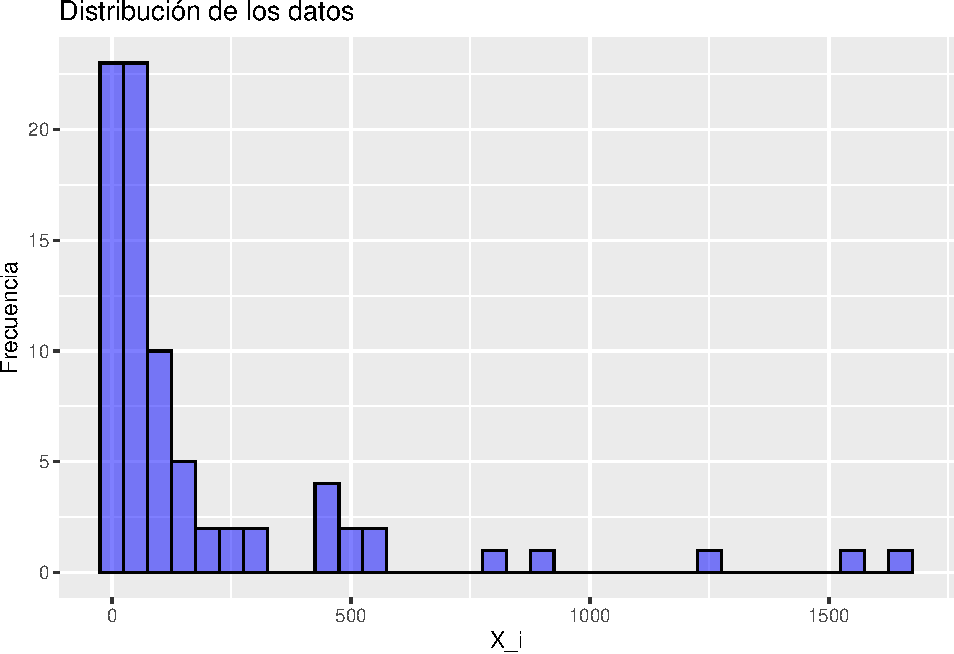
\includegraphics{Extremales_files/figure-latex/unnamed-chunk-12-1.pdf}

\begin{Shaded}
\begin{Highlighting}[]
\CommentTok{\# Parámetros del libro}
\NormalTok{loc\_libro }\OtherTok{\textless{}{-}} \SpecialCharTok{{-}}\FloatTok{6.5}    \CommentTok{\# μ}
\NormalTok{scale\_libro }\OtherTok{\textless{}{-}} \DecValTok{44}     \CommentTok{\# β}
\NormalTok{shape\_libro }\OtherTok{\textless{}{-}} \FloatTok{1.04}   \CommentTok{\# α (parámetro de forma positivo, Fréchet)}

\CommentTok{\# Cálculo de la probabilidad de exceder el valor 50}
\NormalTok{prob\_excede\_50 }\OtherTok{\textless{}{-}} \DecValTok{1} \SpecialCharTok{{-}} \FunctionTok{pgev}\NormalTok{(}\DecValTok{50}\NormalTok{, }\AttributeTok{loc =}\NormalTok{ loc\_libro, }\AttributeTok{scale =}\NormalTok{ scale\_libro, }\AttributeTok{shape =}\NormalTok{ shape\_libro)}

\CommentTok{\# Mostrar la probabilidad de excedencia}
\FunctionTok{print}\NormalTok{(}\FunctionTok{paste}\NormalTok{(}\StringTok{"Probabilidad de excedencia del nivel 50:"}\NormalTok{, }\FunctionTok{round}\NormalTok{(prob\_excede\_50, }\DecValTok{4}\NormalTok{)))}
\end{Highlighting}
\end{Shaded}

\begin{verbatim}
## [1] "Probabilidad de excedencia del nivel 50: 0.3575"
\end{verbatim}

\begin{Shaded}
\begin{Highlighting}[]
\CommentTok{\# Proporción empírica de excedencia del nivel 50}
\NormalTok{prop\_empirica }\OtherTok{\textless{}{-}} \FunctionTok{mean}\NormalTok{(data}\SpecialCharTok{$}\NormalTok{X\_i }\SpecialCharTok{\textgreater{}} \DecValTok{50}\NormalTok{)}
\FunctionTok{print}\NormalTok{(}\FunctionTok{paste}\NormalTok{(}\StringTok{"Proporción empírica de excedencia del nivel 50:"}\NormalTok{, }\FunctionTok{round}\NormalTok{(prop\_empirica, }\DecValTok{4}\NormalTok{)))}
\end{Highlighting}
\end{Shaded}

\begin{verbatim}
## [1] "Proporción empírica de excedencia del nivel 50: 0.5125"
\end{verbatim}

\begin{Shaded}
\begin{Highlighting}[]
\CommentTok{\# Intervalo de confianza para la proporción empírica}
\NormalTok{prop\_ci }\OtherTok{\textless{}{-}} \FunctionTok{prop.test}\NormalTok{(}\FunctionTok{sum}\NormalTok{(data}\SpecialCharTok{$}\NormalTok{X\_i }\SpecialCharTok{\textgreater{}} \DecValTok{50}\NormalTok{), }\FunctionTok{length}\NormalTok{(data}\SpecialCharTok{$}\NormalTok{X\_i))}\SpecialCharTok{$}\NormalTok{conf.int}
\FunctionTok{print}\NormalTok{(}\FunctionTok{paste}\NormalTok{(}\StringTok{"Intervalo de confianza al 95\%:"}\NormalTok{, }\FunctionTok{round}\NormalTok{(prop\_ci[}\DecValTok{1}\NormalTok{], }\DecValTok{3}\NormalTok{), }\StringTok{"{-}"}\NormalTok{, }\FunctionTok{round}\NormalTok{(prop\_ci[}\DecValTok{2}\NormalTok{], }\DecValTok{3}\NormalTok{)))}
\end{Highlighting}
\end{Shaded}

\begin{verbatim}
## [1] "Intervalo de confianza al 95%: 0.399 - 0.625"
\end{verbatim}

\begin{Shaded}
\begin{Highlighting}[]
\FunctionTok{print}\NormalTok{(}\FunctionTok{paste}\NormalTok{(}\StringTok{"Probabilidad de excedencia del nivel 50:"}\NormalTok{, }\FunctionTok{round}\NormalTok{(prob\_excede\_50, }\DecValTok{4}\NormalTok{)))}
\end{Highlighting}
\end{Shaded}

\begin{verbatim}
## [1] "Probabilidad de excedencia del nivel 50: 0.3575"
\end{verbatim}

\begin{Shaded}
\begin{Highlighting}[]
\CommentTok{\# Parámetros del libro}
\NormalTok{loc\_libro }\OtherTok{\textless{}{-}} \SpecialCharTok{{-}}\FloatTok{6.5}    \CommentTok{\# μ}
\NormalTok{scale\_libro }\OtherTok{\textless{}{-}} \DecValTok{44}     \CommentTok{\# β}
\NormalTok{shape\_libro }\OtherTok{\textless{}{-}} \FloatTok{1.04}   \CommentTok{\# α (parámetro de forma positivo, Fréchet)}

\CommentTok{\# Cálculo de la probabilidad de exceder el valor 50}
\NormalTok{prob\_excede\_50 }\OtherTok{\textless{}{-}} \DecValTok{1} \SpecialCharTok{{-}} \FunctionTok{pgev}\NormalTok{(}\DecValTok{50}\NormalTok{, }\AttributeTok{loc =}\NormalTok{ loc\_libro, }\AttributeTok{scale =}\NormalTok{ scale\_libro, }\AttributeTok{shape =}\NormalTok{ shape\_libro)}
\FunctionTok{print}\NormalTok{(}\FunctionTok{paste}\NormalTok{(}\StringTok{"Probabilidad de excedencia del nivel 50:"}\NormalTok{, }\FunctionTok{round}\NormalTok{(prob\_excede\_50, }\DecValTok{4}\NormalTok{)))}
\end{Highlighting}
\end{Shaded}

\begin{verbatim}
## [1] "Probabilidad de excedencia del nivel 50: 0.3575"
\end{verbatim}

\begin{Shaded}
\begin{Highlighting}[]
\CommentTok{\# Parámetros del libro}
\NormalTok{loc\_libro }\OtherTok{\textless{}{-}} \SpecialCharTok{{-}}\FloatTok{6.5}    \CommentTok{\# μ}
\NormalTok{scale\_libro }\OtherTok{\textless{}{-}} \DecValTok{44}     \CommentTok{\# β}
\NormalTok{shape\_libro }\OtherTok{\textless{}{-}} \FloatTok{1.04}   \CommentTok{\# α (parámetro de forma positivo, Fréchet)}

\CommentTok{\# Definir intervalos usando los quintiles empíricos}
\NormalTok{breaks }\OtherTok{\textless{}{-}} \FunctionTok{quantile}\NormalTok{(data}\SpecialCharTok{$}\NormalTok{X\_i, }\AttributeTok{probs =} \FunctionTok{seq}\NormalTok{(}\DecValTok{0}\NormalTok{, }\DecValTok{1}\NormalTok{, }\AttributeTok{length.out =} \DecValTok{6}\NormalTok{))  }\CommentTok{\# 5 intervalos}

\CommentTok{\# Calcular las frecuencias observadas en cada intervalo}
\NormalTok{observed\_counts }\OtherTok{\textless{}{-}} \FunctionTok{hist}\NormalTok{(data}\SpecialCharTok{$}\NormalTok{X\_i, }\AttributeTok{breaks =}\NormalTok{ breaks, }\AttributeTok{plot =} \ConstantTok{FALSE}\NormalTok{)}\SpecialCharTok{$}\NormalTok{counts}

\CommentTok{\# Calcular las probabilidades teóricas en cada intervalo usando la distribución Fréchet ajustada}
\NormalTok{probs }\OtherTok{\textless{}{-}} \FunctionTok{diff}\NormalTok{(}\FunctionTok{pgev}\NormalTok{(breaks, }\AttributeTok{loc =}\NormalTok{ loc\_libro, }\AttributeTok{scale =}\NormalTok{ scale\_libro, }\AttributeTok{shape =}\NormalTok{ shape\_libro))}

\CommentTok{\# Convertir probabilidades en frecuencias esperadas}
\NormalTok{expected\_counts }\OtherTok{\textless{}{-}}\NormalTok{ probs }\SpecialCharTok{*} \FunctionTok{length}\NormalTok{(data}\SpecialCharTok{$}\NormalTok{X\_i)}

\CommentTok{\# Realizar el test de ajuste Chi{-}cuadrado}
\NormalTok{chi\_sq\_test }\OtherTok{\textless{}{-}} \FunctionTok{chisq.test}\NormalTok{(observed\_counts, }\AttributeTok{p =}\NormalTok{ probs, }\AttributeTok{rescale.p =} \ConstantTok{TRUE}\NormalTok{)}

\CommentTok{\# Mostrar los resultados del test}
\FunctionTok{print}\NormalTok{(}\StringTok{"Resultados del test Chi{-}cuadrado con los parámetros del libro:"}\NormalTok{)}
\end{Highlighting}
\end{Shaded}

\begin{verbatim}
## [1] "Resultados del test Chi-cuadrado con los parámetros del libro:"
\end{verbatim}

\begin{Shaded}
\begin{Highlighting}[]
\FunctionTok{print}\NormalTok{(chi\_sq\_test)}
\end{Highlighting}
\end{Shaded}

\begin{verbatim}
## 
##  Chi-squared test for given probabilities
## 
## data:  observed_counts
## X-squared = 4.3938, df = 4, p-value = 0.3553
\end{verbatim}

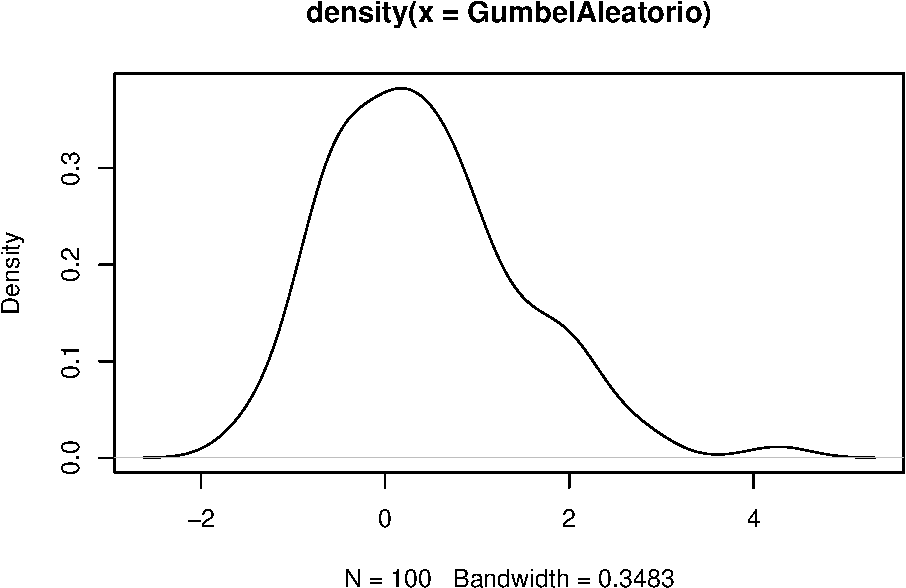
\includegraphics{Extremales_files/figure-latex/unnamed-chunk-18-1.pdf}

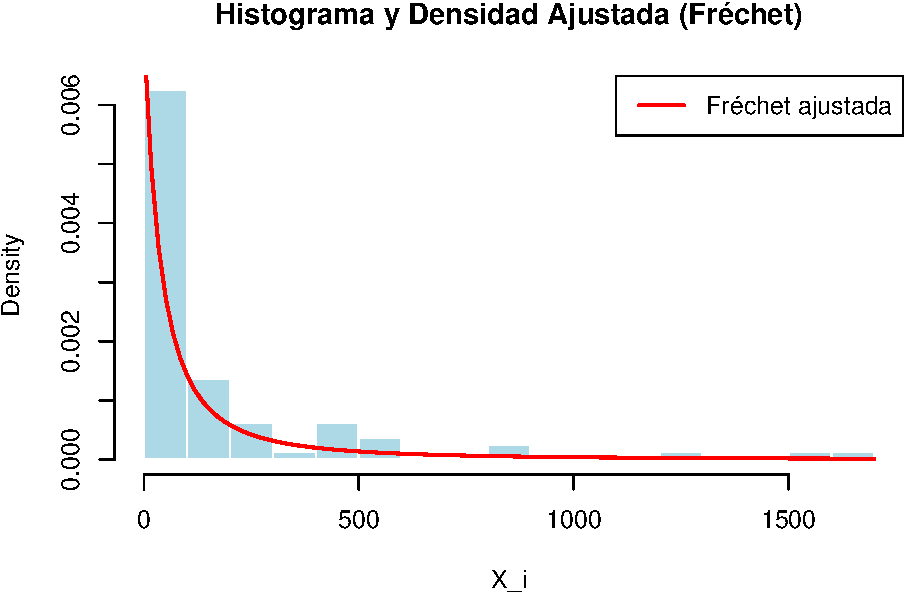
\includegraphics{Extremales_files/figure-latex/unnamed-chunk-19-1.pdf}

\textbf{Observación 10.} Una distribución \(H\) se dice degenerada si \(H(t)=0 \text{ ó } 1\) para todo valor de \(t\). Representan a variables que no son tales, si la distribución de \(X\) es degenerada, entonces \(X\) es una constante, y no tiene sentido
hacer estadística sobre \(X\), por lo tanto sólo tienen
interés para nosotros las distribuciones no-degeneradas.

\section{Distribución Extremal Asintótica}\label{distribuciuxf3n-extremal-asintuxf3tica}

Si \(X_1,...,X_n\) es iid con distribución \(F\) diremos que \(H\) no-degenerada es la Distribución Extremal Asintótica
(DEA) de \(F\)\footnote{De manera equivalente, que \(F\) tiene DEA \(H\).}, si existen dos sucesiones de números reales, \(d_n\) y \(c_n>0\), tales que la distribución de
\begin{equation}
\frac{max(X_1,...,X_n)- d_n}{c_n}\;\text{ tiende a } H \text{ cuando } n \text{ tiende a infinito.}
\end{equation}

\section{Supremo esencial de una variable aleatoria o distribución}\label{supremo-esencial-de-una-variable-aleatoria-o-distribuciuxf3n}

Si \(X\) tiene distribución \(F\),
se llama \(M_X\) al supremo esencial de \(X\) o,
indistintamente, supremo esencial de \(F\) (denotado
\(M_F\)) a

\begin{equation}
M_X = M_F = \sup\{t \; / \; F(t) < 1\}
\end{equation}

\textbf{Observación 11.}

\begin{itemize}
\tightlist
\item
  Si \(F\) es \(U(a,b)\), \(M_F=b\).
\item
  Si \(F\) es \(Bin(m,p)\), \(M_F=m\).
\item
  Si \(F\) es Normal, Exponencial, Cauchy o Poisson entonces \(M_F\) es infinito.
\end{itemize}

\textbf{Teorema 4:} Si \(X_1,...,X_n\) iid con distribución \(F\) cualquiera, entonces, para \(n \rightarrow \infty\),

\begin{equation}
X_n^{\ast} =max(X_1,...,X_n) \rightarrow M_F
\end{equation}

\textbf{Observación 12.} El resultado anterior vale
incluso si \(M_F\) es infinito, pero si \(M_F\) es finito, como
\(Xn* - Mf\) tiende a cero, por analogía con el Teorema
Central del Límite para promedios, buscaríamos
una sucesión \(c_n>0\) y que tienda a cero de modo tal
que \((X_n^{\ast}- M_F )/ c_n\) tienda a una distribución no-
degenerada y de allí surge buscar la DEA.

\textbf{Teorema 5:} Si \(F\) es una distribución con \(M_F\) finito, y para \(X\) con distribución \(F\) se cumple que
\begin{equation}
P(X=M_F)>0
\end{equation}
entonces \(F\) no admite DEA.

\textbf{Observación 13.} Si \(F\) es \(Bin(m,p) \Rightarrow M_F=m\). Si \(X\)
tiene distribución \(F\), entonces
\(P( X=M_F)= P( X=m)= p^m>0\),
asi que la distribucion \(Bin(m,p)\) NO admite DEA,
no se puede aproximar la distribución del máximo
de una muestra iid de variables \(Bin(m,p)\).

El Teorema anterior es un caso particular del
próximo.

\textbf{Teorema 6:} Si \(F\) es una distribución con \(M_F\) finito o infinito que
admite DEA, y \(X\) tiene distribución \(F\), entonces el
limite cuando \(t\) tiende a \(M_F\) por izquierda de

\begin{equation}
P(X>t)/P(X \leq t)
\end{equation}

debe ser 1.

\textbf{Observación 13.} Si \(F\) es una distribución de
Poisson de parámetro \(\lambda >0\), \(M_F\) es infinito. Si \(k\) es un
natural, entonces

\begin{align}
P(X>t)/P(X \leq t)& = P(X \leq k+1)/P(X \leq k)\\
& = 1-\left\{ P(X=k)/P(X \leq k) \right\} \approx 1-(1- \lambda/k)
\end{align}

que tiende a 0 cuando \(k\) tiende a infinito, por lo
cual \(F\) NO admite DEA, o sea que no se puede aproximar el máximo de una sucesión iid de variables de Poisson.

\textbf{Observación 14.} El Teorema 6 brinda una
condición NECESARIA pero NO SUFICIENTE
para DEA. Un ejemplo de ello lo aportó Von Mises,
mostrando que la distribución

\begin{equation}
F(x)= 1- e^{(-x-\sin(x))}
\end{equation}

cumple con la condicion del Teorema 6 pero no
admite DEA. El tema será cerrado al estudiar los
dominios de atracción maximal, en breve.

Veamos ahora ejemplos donde la DEA resulta
aplicable y que ratifican algunos hechos que
anticipáramos.

\textbf{Observación 15.} Si \(F\) es \(U(0,1)\) y consideramos
\(X_1,...,X_n\) iid con distribución \(F\), resulta que
la distribución de \(n( X_n^{\ast} - 1)\) tiende a \(\Psi_1\) por lo cual la distribución uniforme tiene DEA
Weibull.

\textbf{Observación 16.} Si \(F\) es Exponencial de
parámetro 1 y consideramos \(X_1,...,X_n\) iid con
distribución \(F\), se tiene que la distribución de \(X_n^{\ast} - \log n\) tiende a \(\Lambda\) por lo cual la distribución exponencial tiene DEA Gumbel.

\textbf{Observación 17.} Si \(F\) es \(N(0,1)\) y consideramos
\(X_1,...,X_n\) iid con distribución \(F\), definimos la función continua y estrictamente decreciente (para \(u>0\))

\begin{equation}
g(u)= \frac{e^{-u^2/4\pi}}{u}.
\end{equation}

Como \(\lim_{u \to 0}\; g(u) \rightarrow \infty\) y \(\lim_{u \to \infty}\; g(u) \rightarrow 0\),
para todo natural \(n\) existe un único valor \(u_n\) tal que

\begin{equation}
g(u_n)=\frac{1}{n}
\end{equation}

y resulta que \(\frac{u_n}{\sqrt{2\pi} (X_n^{\ast}- u_n /\sqrt 2\pi)} \rightarrow \Lambda\), por lo cual la distribución normal tiene DEA Gumbel.

\textbf{Observación 18.} Si \(F\) es Cauchy standard que se expresa como \(C(0,1)\)
y consideramos \(X_1,...,X_n\) iid con distribución \(F\), se tiene que
la distribución de \(\pi X_n^{\ast}/n\) tiende a \(F_1\) por lo cual la distribución Cauchy tiene DEA Fréchet.

Los ejemplos anteriores no son sorprendentes, en el sentido
que aunque presentamos FTG en una versión simplificada,
dicho teorema sugiere que cuando \(F\) admite DEA, la
distribución \(H\) deberá ser una distribución extremal. De hecho
FTG resulta de combinar dos teoremas, basadas en una nueva
definición, la de distribución \textbf{max-estable}.

\section{Distribución max-estables}\label{distribuciuxf3n-max-estables}

Si dada \(F\) distribución, \(X\) con distribución \(F\), \(k\) natural
arbitrario y \(X_1,...,X_k\) iid con distribución \(F\), existen
reales \(a_k, b_k\) tales que \(max(X_1,...,X_k)\) tiene la misma
distribución que \(a_k X+ b_k\), \(F\) se dice max-estable.

El Teorema FTG resulta de superponer los dos
siguientes teoremas.

\textbf{Teorema 7:}

\begin{enumerate}
\def\labelenumi{\alph{enumi})}
\item
  Si \(F\) admite DEA \(H\), entonces \(H\) es max-estable.
\item
  Si \(H\) es max-estable, es la DEA de sí misma.
\end{enumerate}

\textbf{Teorema 8:}

Una distribución es max-estable si y solo si es extremal: Gumbel, Weibull, Fréchet.

El Teorema 7 es bastante intuitivo y análogo a los
teoremas de Lévy sobre distribuciones estables en
aproximaciones asintóticas de las distribuciones de
sumas. Para el Teorema 8 haremos enseguida un
ejercicio sencillo que nos ayudará a hacerlo creíble.

Luego precisaremos, para terminar con esta parte,
cómo son las distribuciones que tienen por DEA
cada uno de los tres tipos de distribuciones
extremales. Para eso precisamos recordar algunas
definiciones, como la siguiente.

\textbf{Observación 19.} Si \(F\) y \(G\) son dos distribuciones,
tienen colas equivalentes si \(M_F=M_G\) y cuando \(t\)
tiende a \(M_F\) por izquierda, \((1-F(t))/(1-G(t))\) tiende a
un valor \(c>0\).

Recordando ahora cómo se calcula la distribución
del máximo de dos variables independientes, es
muy sencillo calcular la distribución del \(max\left\{ X,Y \right\}\),
cuando \(X\) e \(Y\) son independientes y cada una de
ellas es una distribución extremal. Se tiene el
siguiente resultado.

\begin{longtable}[]{@{}
  >{\raggedright\arraybackslash}p{(\columnwidth - 4\tabcolsep) * \real{0.2500}}
  >{\raggedright\arraybackslash}p{(\columnwidth - 4\tabcolsep) * \real{0.2500}}
  >{\raggedright\arraybackslash}p{(\columnwidth - 4\tabcolsep) * \real{0.5000}}@{}}
\toprule\noalign{}
\begin{minipage}[b]{\linewidth}\raggedright
\(X\)
\end{minipage} & \begin{minipage}[b]{\linewidth}\raggedright
\(Y\)
\end{minipage} & \begin{minipage}[b]{\linewidth}\raggedright
\(max(X,Y)\)
\end{minipage} \\
\midrule\noalign{}
\endhead
\bottomrule\noalign{}
\endlastfoot
\textcolor{red}{Weibull} & \textcolor{red}{Weibull} & \textcolor{red}{Weibull} \\
\textcolor[rgb]{0.0,0.5,0.0}{Weibull} & \textcolor[rgb]{0.0,0.5,0.0}{Gumbel} & \textcolor[rgb]{0.0,0.5,0.0}{Cola equivalente Gumbel} \\
\textcolor{blue}{Weibull} & \textcolor{blue}{Fréchet} & \textcolor{blue}{Fréchet} \\
\textcolor[rgb]{0.0,0.5,0.0}{Gumbel} & \textcolor[rgb]{0.0,0.5,0.0}{Weibull} & \textcolor[rgb]{0.0,0.5,0.0}{Cola equivalente Gumbel} \\
\textcolor{red}{Gumbel} & \textcolor{red}{Gumbel} & \textcolor{red}{Gumbel} \\
\textcolor{blue}{Gumbel} & \textcolor{blue}{Fréchet} & \textcolor{blue}{Cola equivalente Fréchet} \\
\textcolor{blue}{Fréchet} & \textcolor{blue}{Weibull} & \textcolor{blue}{Fréchet} \\
\textcolor{blue}{Fréchet} & \textcolor{blue}{Gumbel} & \textcolor{blue}{Cola equivalente Fréchet} \\
\textcolor{red}{Fréchet} & \textcolor{red}{Fréchet} & \textcolor{red}{Fréchet} \\
\end{longtable}

\textcolor{red}{\rule{1em}{1em} Las extremales son max-estables: tomar máximos de dos del mismo tipo queda en el mismo tipo.}

\textcolor[rgb]{0.0,0.5,0.0}{\rule{1em}{1em} Gumbel es más pesada que Weibull. En la cola, que es lo que cuenta para máximos, prima Gumbel.}

\textcolor{blue}{\rule{1em}{1em} Fréchet es más pesada que Gumbel y mucho más pesada que Weibull.}

\subsection{Ejemplos de libro}\label{ejemplos-de-libro}

Ejemplos de \citet{coles2001introduction} con el paquete \citet{ismev2020} :

\subsubsection{POT}\label{pot}

\begin{figure}

{\centering 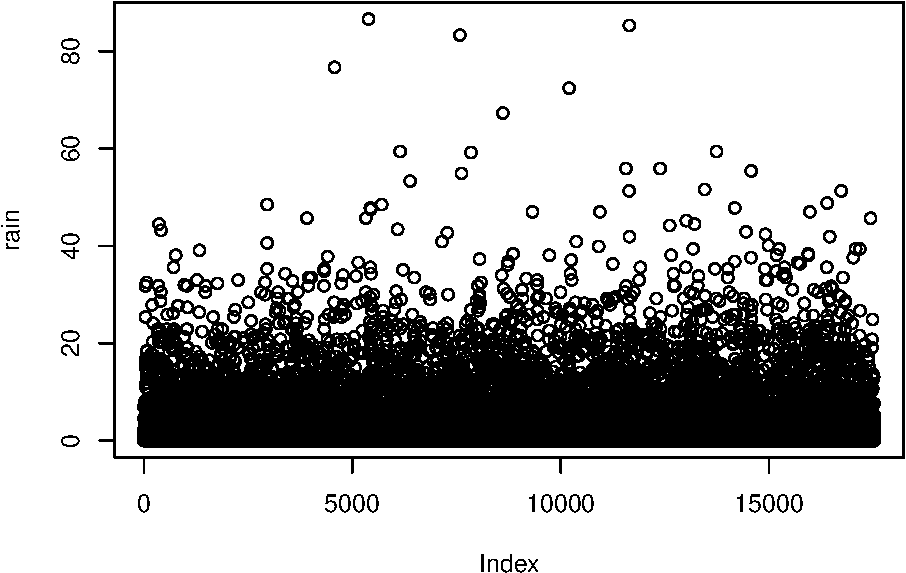
\includegraphics[width=0.8\linewidth,alt={Acumulaciones diarias de lluvia en una ubicación en el suroeste de Inglaterra registradas durante el período 1914-1962.}]{Extremales_files/figure-latex/nice-fig3-1} 

}

\caption{Acumulaciones diarias de lluvia en una ubicación en el suroeste de Inglaterra registradas durante el período 1914-1962.}\label{fig:nice-fig3}
\end{figure}

Considerando la Figura \ref{fig:nice-fig3}, podemos definir un evento como extremo si supera un cierto nivel alto, quizás una precipitación diaria de \(30\; mm\) en este caso. Entonces, los valores extremos son ahora aquellas observaciones que superan un cierto umbral alto (\citet{coles2001introduction}).

\chapter{\texorpdfstring{Un primer enfoque de datos no \(iid\)}{Un primer enfoque de datos no iid}}\label{cross}

\section{Análisis de series temporales}\label{anuxe1lisis-de-series-temporales}

\section{Pruebas de raíz unitaria y tendencia}\label{pruebas-de-rauxedz-unitaria-y-tendencia}

\subsection{Concepto de Estacionariedad}\label{concepto-de-estacionariedad}

\begin{Shaded}
\begin{Highlighting}[]
\FunctionTok{head}\NormalTok{(portpirie)}
\end{Highlighting}
\end{Shaded}

\begin{verbatim}
## [1] 4.03 3.83 3.65 3.88 4.01 4.08
\end{verbatim}

\begin{figure}

{\centering 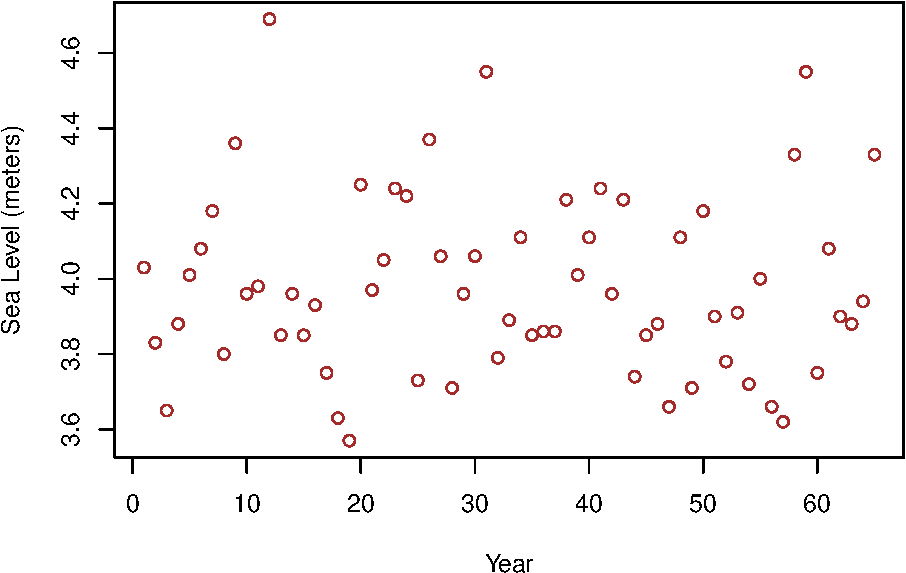
\includegraphics[width=0.8\linewidth,alt={Niveles máximos anuales del nivel del mar registrados en Port Pirie, una localidad justo al norte de Adelaida, Australia del Sur, durante el período 1923-1987}]{Extremales_files/figure-latex/nice-fig2-1} 

}

\caption{Niveles máximos anuales del nivel del mar registrados en Port Pirie.}\label{fig:nice-fig2}
\end{figure}

La figura \ref{fig:nice-fig2} muestra los niveles máximos anuales del nivel del mar registrados en Port Pirie, una localidad justo al norte de Adelaida, Australia del Sur, durante el período 1923-1987. A partir de estos datos, puede ser necesario estimar el nivel máximo del mar que probablemente ocurra en la región en los próximos 100 o 1000 años. Esto plantea una cuestión importante: ¿cómo podemos estimar los niveles que pueden ocurrir en los próximos 1000 años sin conocer, por ejemplo, los cambios climáticos que podrían suceder?

No hay evidencia contundente en la figura que sugiera que el patrón de variación en los niveles del mar haya cambiado durante el período de observación, pero dicha estabilidad podría no persistir en el futuro. Esta advertencia es crucial: aunque la teoría de valores extremos ha adoptado terminología como el ``nivel de retorno a 1000 años'', que corresponde al nivel que se espera que sea excedido exactamente una vez en los próximos 1000 años, esto solo tiene sentido bajo el supuesto de estabilidad (o estacionariedad) en el proceso subyacente. Es más realista hablar en términos de niveles que, bajo las condiciones actuales, ocurrirán en un año determinado con una baja probabilidad (\citet{coles2001introduction}).

\subsubsection{Ejemplo en Finanzas}\label{ejemplo-en-finanzas}

Las técnicas de valores extremos han ganado popularidad en aplicaciones financieras. Esto no es sorprendente: la solvencia financiera de una inversión probablemente esté determinada por cambios extremos en las condiciones del mercado en lugar de cambios típicos. Sin embargo, la compleja estructura estocástica de los mercados financieros implica que la aplicación ingenua de técnicas de valores extremos puede ser engañosa (\citet{coles2001introduction}).

\begin{Shaded}
\begin{Highlighting}[]
\FunctionTok{data}\NormalTok{(dowjones)}
\NormalTok{dowjones}\SpecialCharTok{$}\NormalTok{LogDiff }\OtherTok{\textless{}{-}} \FunctionTok{c}\NormalTok{(}\ConstantTok{NA}\NormalTok{, }\FunctionTok{diff}\NormalTok{(}\FunctionTok{log}\NormalTok{(dowjones}\SpecialCharTok{$}\NormalTok{Index)))}
\end{Highlighting}
\end{Shaded}

\begin{Shaded}
\begin{Highlighting}[]
\FunctionTok{head}\NormalTok{(dowjones)}
\end{Highlighting}
\end{Shaded}

\begin{verbatim}
##                  Date   Index       LogDiff
## 1 1995-09-11 02:00:00 4704.94            NA
## 2 1995-09-12 02:00:00 4747.21  0.0089440565
## 3 1995-09-13 02:00:00 4765.52  0.0038495832
## 4 1995-09-14 02:00:00 4801.80  0.0075841874
## 5 1995-09-15 02:00:00 4797.57 -0.0008813079
## 6 1995-09-18 02:00:00 4780.41 -0.0035832228
\end{verbatim}

\begin{figure}

{\centering 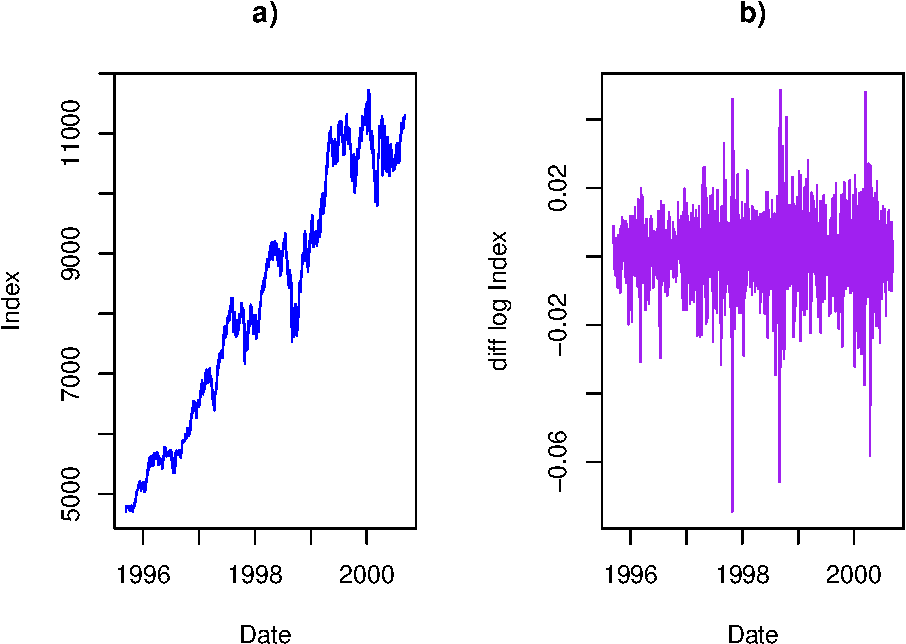
\includegraphics[width=0.8\linewidth,alt={Panel izquierdo: precios de cierre diario del índice Dow Jones.Panel derecho: rendimientos logarítmicos diarios del índice Dow Jones.}]{Extremales_files/figure-latex/nice-fig4-1} 

}

\caption{Panel a) Precios de cierre diario del índice Dow Jones. Panel b) Rendimientos diarios del índice Dow Jones (en logarítmos).}\label{fig:nice-fig4}
\end{figure}

La Fig.\ref{fig:nice-fig4} muestra los precios de cierre diario del índice Dow Jones durante un período de 5 años. Evidentemente, el nivel del proceso ha cambiado drásticamente a lo largo del período observado, y las cuestiones sobre los valores extremos del comportamiento diario quedan eclipsadas por la variación temporal a largo plazo en la serie. Varios estudios empíricos sobre series de este tipo han indicado que se puede obtener una aproximación a la estacionariedad tomando los logaritmos de los cocientes de observaciones sucesivas, lo que se conoce como los retornos logarítmicos diarios. El panel b) de la Fig. \ref{fig:nice-fig4} sugiere una transformación razonablemente exitosa hacia la estacionariedad. El análisis de las propiedades de valores extremos de dichas series transformadas puede proporcionar a los analistas financieros información clave sobre el mercado (\citet{coles2001introduction}).

\chapter{Parts}\label{parts}

You can add parts to organize one or more book chapters together. Parts can be inserted at the top of an .Rmd file, before the first-level chapter heading in that same file.

Add a numbered part: \texttt{\#\ (PART)\ Act\ one\ \{-\}} (followed by \texttt{\#\ A\ chapter})

Add an unnumbered part: \texttt{\#\ (PART\textbackslash{}*)\ Act\ one\ \{-\}} (followed by \texttt{\#\ A\ chapter})

Add an appendix as a special kind of un-numbered part: \texttt{\#\ (APPENDIX)\ Other\ stuff\ \{-\}} (followed by \texttt{\#\ A\ chapter}). Chapters in an appendix are prepended with letters instead of numbers.

\chapter{Footnotes and citations}\label{footnotes-and-citations}

\section{Footnotes}\label{footnotes}

Footnotes are put inside the square brackets after a caret \texttt{\^{}{[}{]}}. Like this one \footnote{This is a footnote.}.

\section{Citations}\label{citations}

Reference items in your bibliography file(s) using \texttt{@key}.

For example, we are using the \textbf{bookdown} package \citep{R-bookdown} (check out the last code chunk in index.Rmd to see how this citation key was added) in this sample book, which was built on top of R Markdown and \textbf{knitr} \citep{xie2015} (this citation was added manually in an external file book.bib).
Note that the \texttt{.bib} files need to be listed in the index.Rmd with the YAML \texttt{bibliography} key.

The RStudio Visual Markdown Editor can also make it easier to insert citations: \url{https://rstudio.github.io/visual-markdown-editing/\#/citations}

\chapter{Blocks}\label{blocks}

\section{Equations}\label{equations}

Here is an equation.

\begin{equation} 
  f\left(k\right) = \binom{n}{k} p^k\left(1-p\right)^{n-k}
  \label{eq:binom}
\end{equation}

You may refer to using \texttt{\textbackslash{}@ref(eq:binom)}, like see Equation \eqref{eq:binom}.

\section{Theorems and proofs}\label{theorems-and-proofs}

Labeled theorems can be referenced in text using \texttt{\textbackslash{}@ref(thm:tri)}, for example, check out this smart theorem \ref{thm:tri}.

\begin{theorem}
\protect\hypertarget{thm:tri}{}\label{thm:tri}For a right triangle, if \(c\) denotes the \emph{length} of the hypotenuse
and \(a\) and \(b\) denote the lengths of the \textbf{other} two sides, we have
\[a^2 + b^2 = c^2\]
\end{theorem}

Read more here \url{https://bookdown.org/yihui/bookdown/markdown-extensions-by-bookdown.html}.

\section{Callout blocks}\label{callout-blocks}

The R Markdown Cookbook provides more help on how to use custom blocks to design your own callouts: \url{https://bookdown.org/yihui/rmarkdown-cookbook/custom-blocks.html}

\section{Referencias cruzadas}\label{referencias-cruzadas}

There are two steps to cross-reference any heading:

\begin{enumerate}
\def\labelenumi{\arabic{enumi}.}
\tightlist
\item
  Label the heading: \texttt{\#\ Hello\ world\ \{\#nice-label\}}.

  \begin{itemize}
  \tightlist
  \item
    Leave the label off if you like the automated heading generated based on your heading title: for example, \texttt{\#\ Hello\ world} = \texttt{\#\ Hello\ world\ \{\#hello-world\}}.
  \item
    To label an un-numbered heading, use: \texttt{\#\ Hello\ world\ \{-\#nice-label\}} or \texttt{\{\#\ Hello\ world\ .unnumbered\}}.
  \end{itemize}
\item
  Next, reference the labeled heading anywhere in the text using \texttt{\textbackslash{}@ref(nice-label)}; for example, please see Chapter \ref{cross}.

  \begin{itemize}
  \tightlist
  \item
    If you prefer text as the link instead of a numbered reference use: \hyperref[cross]{any text you want can go here}.
  \end{itemize}
\end{enumerate}

Figures and tables \emph{with captions} can also be cross-referenced from elsewhere in your book using \texttt{\textbackslash{}@ref(fig:chunk-label)} and \texttt{\textbackslash{}@ref(tab:chunk-label)}, respectively.

See Figure \ref{fig:nice-fig}.

\begin{Shaded}
\begin{Highlighting}[]
\FunctionTok{par}\NormalTok{(}\AttributeTok{mar =} \FunctionTok{c}\NormalTok{(}\DecValTok{4}\NormalTok{, }\DecValTok{4}\NormalTok{, .}\DecValTok{1}\NormalTok{, .}\DecValTok{1}\NormalTok{))}
\FunctionTok{plot}\NormalTok{(pressure, }\AttributeTok{type =} \StringTok{\textquotesingle{}b\textquotesingle{}}\NormalTok{, }\AttributeTok{pch =} \DecValTok{19}\NormalTok{)}
\end{Highlighting}
\end{Shaded}

\begin{figure}

{\centering 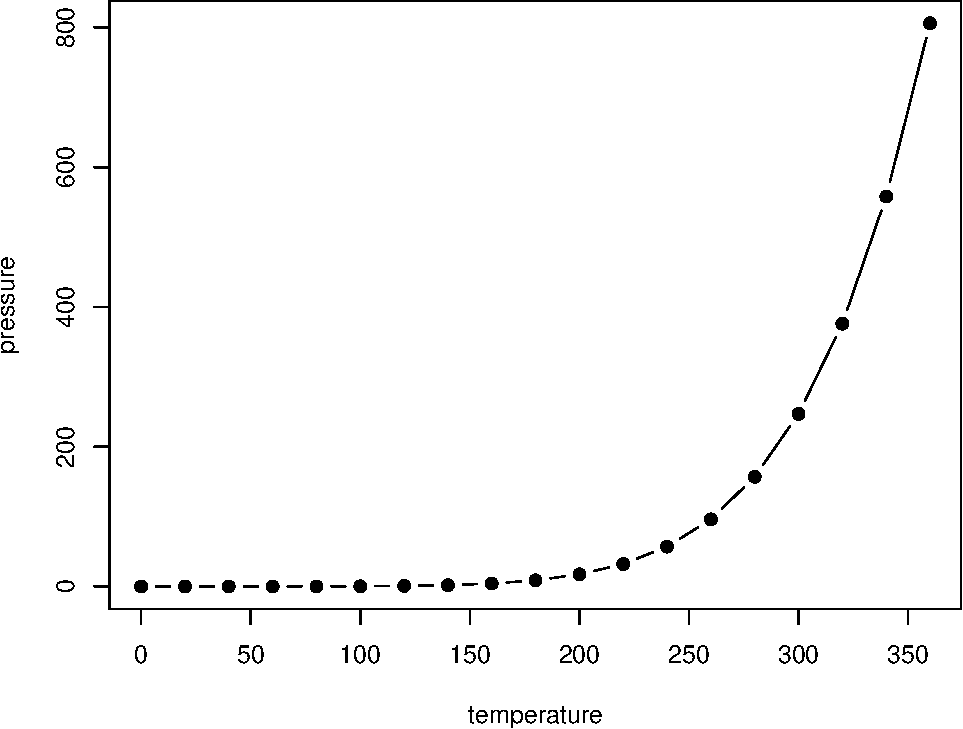
\includegraphics[width=0.8\linewidth,alt={Plot with connected points showing that vapor pressure of mercury increases exponentially as temperature increases.}]{Extremales_files/figure-latex/nice-fig-1} 

}

\caption{Here is a nice figure!}\label{fig:nice-fig}
\end{figure}

Don't miss Table \ref{tab:nice-tab}.

\begin{Shaded}
\begin{Highlighting}[]
\NormalTok{knitr}\SpecialCharTok{::}\FunctionTok{kable}\NormalTok{(}
  \FunctionTok{head}\NormalTok{(pressure, }\DecValTok{10}\NormalTok{), }\AttributeTok{caption =} \StringTok{\textquotesingle{}Here is a nice table!\textquotesingle{}}\NormalTok{,}
  \AttributeTok{booktabs =} \ConstantTok{TRUE}
\NormalTok{)}
\end{Highlighting}
\end{Shaded}

\begin{table}

\caption{\label{tab:nice-tab}Here is a nice table!}
\centering
\begin{tabular}[t]{rr}
\toprule
temperature & pressure\\
\midrule
0 & 0.0002\\
20 & 0.0012\\
40 & 0.0060\\
60 & 0.0300\\
80 & 0.0900\\
\addlinespace
100 & 0.2700\\
120 & 0.7500\\
140 & 1.8500\\
160 & 4.2000\\
180 & 8.8000\\
\bottomrule
\end{tabular}
\end{table}

\chapter{Sharing your book}\label{sharing-your-book}

\section{Publishing}\label{publishing}

HTML books can be published online, see: \url{https://bookdown.org/yihui/bookdown/publishing.html}

\section{404 pages}\label{pages}

By default, users will be directed to a 404 page if they try to access a webpage that cannot be found. If you'd like to customize your 404 page instead of using the default, you may add either a \texttt{\_404.Rmd} or \texttt{\_404.md} file to your project root and use code and/or Markdown syntax.

\section{Metadata for sharing}\label{metadata-for-sharing}

Bookdown HTML books will provide HTML metadata for social sharing on platforms like Twitter, Facebook, and LinkedIn, using information you provide in the \texttt{index.Rmd} YAML. To setup, set the \texttt{url} for your book and the path to your \texttt{cover-image} file. Your book's \texttt{title} and \texttt{description} are also used.

This \texttt{gitbook} uses the same social sharing data across all chapters in your book- all links shared will look the same.

Specify your book's source repository on GitHub using the \texttt{edit} key under the configuration options in the \texttt{\_output.yml} file, which allows users to suggest an edit by linking to a chapter's source file.

Read more about the features of this output format here:

\url{https://pkgs.rstudio.com/bookdown/reference/gitbook.html}

Or use:

\begin{Shaded}
\begin{Highlighting}[]
\NormalTok{?bookdown}\SpecialCharTok{::}\NormalTok{gitbook}
\end{Highlighting}
\end{Shaded}


  \bibliography{book.bib,packages.bib}

\end{document}
